\documentclass[12pt, a4paper, oneside]{ctexart}
\usepackage[hyphenbreaks]{breakurl}
\usepackage[hyphens]{url}
\usepackage{amsmath, amsthm, amssymb, appendix, bm, graphicx, hyperref, mathrsfs, color, tikz}
\usetikzlibrary{shapes,arrows}

\makeatletter
\def\UrlAlphabet{%
    \do\a\do\b\do\c\do\d\do\e\do\f\do\g\do\h\do\i\do\j%
    \do\k\do\l\do\m\do\n\do\o\do\p\do\q\do\r\do\s\do\t%
    \do\u\do\v\do\w\do\x\do\y\do\z\do\A\do\B\do\C\do\D%
    \do\E\do\F\do\G\do\H\do\I\do\J\do\K\do\L\do\M\do\N%
    \do\O\do\P\do\Q\do\R\do\S\do\T\do\U\do\V\do\W\do\X%
    \do\Y\do\Z}
\def\UrlDigits{\do\1\do\2\do\3\do\4\do\5\do\6\do\7\do\8\do\9\do\0}
\g@addto@macro{\UrlBreaks}{\UrlOrds}
\g@addto@macro{\UrlBreaks}{\UrlAlphabet}
\g@addto@macro{\UrlBreaks}{\UrlDigits}
\makeatother

\tikzstyle{startstop} = [rectangle,rounded corners, minimum width=3cm,minimum height=1cm,text centered, draw=black,fill=red!30]
\tikzstyle{io} = [trapezium, trapezium left angle = 70,trapezium right angle=110,minimum width=3cm,minimum height=1cm,text centered,draw=black,fill=blue!30]
\tikzstyle{process} = [rectangle,minimum width=3cm,minimum height=1cm,text centered,text width =3cm,draw=black,fill=orange!30]
\tikzstyle{decision} = [diamond,minimum width=3cm,minimum height=1cm,text centered,draw=black,fill=green!30]
\tikzstyle{arrow} = [thick,->,>=stealth]

\title{\textbf{论文阅读笔记}}
\author{知行合一}
\date{\today}
\linespread{1.5}
\newtheorem{theorem}{定理}[section]
\newtheorem{definition}[theorem]{定义}
\newtheorem{lemma}[theorem]{引理}
\newtheorem{corollary}[theorem]{推论}
\newtheorem{example}[theorem]{例}
\newtheorem{proposition}[theorem]{命题}
\renewcommand{\abstractname}{\Large\textbf{摘要}}
\hypersetup{
    colorlinks=true,
    linkcolor=black
}

\begin{document}

    \maketitle

    \setcounter{page}{0}
    \maketitle
    \thispagestyle{empty}


    \begin{abstract}
        4.1、4.3与4.4这3篇工作,均在NSD数据集上进行从fMRI到自然场景的视觉图像的重建工作。4.6、4.7、4.8这3篇工作均在algonauts的2023挑战赛数据集上进行的从自然场景到fMRI体素的预测工作,该三篇文章为该挑战赛目前的前三名。

        神经编码与神经解码。编码:建立机理模型,一个刺激如何造成一种响应模式?解码:重建大脑在做的事,这些响应告诉我们关于刺激的什么信息?视觉编码模型的医疗意义:为研制视网膜假体提供理论基础、脑机接口和测谎仪。

    \noindent\textbf{关键词:}视觉编码的可解释性研究.
    \end{abstract}


    \newpage
    \pagenumbering{Roman}
    \setcounter{page}{1}
    \tableofcontents
    \newpage
    \setcounter{page}{1}
    \pagenumbering{arabic}

    % 第一节: 沈向洋读技术类论文的10个问题
    \section{沈向洋技术类论文十问}
    \noindent(1).论文试图解决什么问题?\\
    (2).这是否是一个新的问题?\\
    (3).这篇文章要验证一个什么科学假设?\\
    (4).有哪些相关研究?如何归类?谁是这一领域值得关注的研究员?\\
    (5).论文中提到的解决方案之关键是什么?\\
    (6).论文中的实验是如何设计的?\\
    (7).用于定量评估的数据集是什么?代码有没有开源?\\
    (8).论文中的实验及结果有没有很好地支撑需要验证的科学假设?\\
    (9).这篇论文到底有什么贡献?\\
    (10).下一步呢?有什么工作可以继续深入?\\

    % 第二节: 收录多种数据集和编程工具箱
    \section{数据集和工具箱}
    \subsection{OpenNeuro}
    \noindent网址:\url{https://openneuro.org}\\
    使用指南:\url{https://docs.openneuro.org/user_guide.html}\\
    翻墙:不需要\\
    更新:众多数据集,会持续更新\\
    数据集模态:MRI(核磁共振)、PET(正电子发射断层扫描)、EEG(脑电图)、iEEG(颅内脑电图)、MEG(脑磁图)\\
    搜索功能:支持

    \subsection{Allen Brain Map}
    \noindent网址:\url{https://portal.brain-map.org}\\
    简介概述:\url{https://portal.brain-map.org/explore/overview}\\
    翻墙:不需要\\
    更新:数据集和工具箱,会持续更新\\
    搜索功能:不支持自定义单词搜索,但是可以加标签检索

    \subsection{CRCNS}
    \noindent全称:Collaborative Research in Computational Neuroscience \\
    网址:\url{https://crcns.org}\\
    简介概述:\url{https://crcns.org/download}\\
    翻墙:不需要\\
    更新:News一栏基本停留在2018年\\
    搜索功能:支持。数据按照树状目录结构排列。

    \subsection{NeuroRA}
    \noindent网址:\url{https://neurora.github.io/NeuroRA/}\\
    简介概述:基于Python的处理神经数据的工具箱\\
    文档:\url{https://neurora.github.io/documentation/index.html}\\
    翻墙:不需要\\
    安装:pip install neurora

    \subsection{Brainlife}
    \noindent网址:\url{https://brainlife.io/about/}\\
    简介概述:神经科学数据分析平台\\
    翻墙:不需要\\
    文档:\url{https://brainlife.io/docs/}

    \subsection{PyMVPA}
    \noindent网址:\url{http://www.pymvpa.org/}\\
    简介概述:Multi-Variate Pattern Analysis (MVPA) in Python.适用于统计学习分析处理的工具。

    \subsection{Easy fMRI}
    \noindent网址:\url{https://easyfmri.learningbymachine.com/}\\
    简介概述:支持GPU的用于人脑映射和解码的的工具箱。

    \subsection{Natural Scenes Dataset数据集\cite{Allen2022}}
    \noindent网址:\url{http://naturalscenesdataset.org/}\\
    简介:\url{https://cvnlab.slite.page/p/AGEte5w9Nq/Overview-of-the-data}\\
    下载指令:aws s3 sync [--no-sign-request] s3://natural-scenes-dataset/子集名称 本地路径\\
    注意:必须要有亚马逊账号,否则下载的数据有问题。\\
    8名受试者,1.8mm分辨率全脑7TfMRI。子集的名称和含义见表\ref{subset}。

    \begin{table}[ptbp]
        \begin{center}
            \caption{子集的名称、大小与含义}
            \label{subset}
            \begin{tabular}{c|c|c} % l c r分别表示左对齐、居中、右对齐
                \textbf{名称} & \textbf{大小} & \textbf{含义}\\
                \hline
                nsddata & 49GB & 基本数据文件的主目录\\
                nsddata\_betas & 8.3TB
                & 估测fMRI单次相应(β)\\
                nsddata\_stimuli & 40GB & 包含了实验中的彩色自然场景图像\\
                nsddata\_timeseries & 3.4TB & 包含预处理的fMRI时间序列数据\\
                nsddata\_other & 25GB & 包含用于运行实验的材料和没有经过编辑的FreeSufer输出\\
                nsddata\_diffusion & 200GB & 分析扩散数据的derivatives \\
                nsddata\_rawdata & 946GB & 包含BIDS格式的原始数据
            \end{tabular}
        \end{center}
    \end{table}

    \subsection{Algonauts Project 2023: Brain Data}
    \noindent网址:\url{http://algonauts.csail.mit.edu/challenge.html}\\
    下载地址:\url{https://drive.google.com/drive/folders/17RyBAnvDhrrt18Js2VZqSVi_nZ7bn3G3}\\
    代码教程:\url{https://colab.research.google.com/drive/1bLJGP3bAo_hAOwZPHpiSHKlt97X9xsUw?usp=share_link#scrollTo=DxkcThGURffq}\\
    \textbf{训练数据:}

    Images:8名受试者分别观看了[9841, 9841, 9082, 8779, 9841, 9082, 9841, 8779]张不同的png格式的图像。例如,受试者1的第一个训练图像被命名为“train-0001\_nsd-00013.png”。第一个索引(“train-0001”)对图像进行排序,以匹配fMRI训练分割数据的刺激图像维度。此索引从1开始。第二个索引('nsd-00013')对应73000个nsd图像ID,您可以使用这些ID将图像映射回原始的'.hdf5'nsd图像文件(其中包含nsd实验中使用的所有73000个图像),并从那里映射到COCO数据集图像以获取元数据)

    fMRI:左半球(LH)和右半球(RH)文件分别由19004个和20544个顶点组成,由于数据丢失,受试者6(18978个LH和20220个RH顶点)和8(18981个LH和20530个右侧顶点)除外。

    \noindent\textbf{测试数据:}

    Images:8名受试者分别观看了[159, 159, 293, 395, 159, 293, 159, 395]张不同的png格式的图像。

    fMRI:该数据集未发布(该比赛的重建目标)

    \noindent\textbf{视皮层的不同功能的兴趣区域(Region-of-Interest, ROI):}

    注意:并非所有的ROI都存在于每个受试者中。

    \begin{itemize}
        \item[$\bullet$]Early retinotopic visual regions(prf-visualrois):V1v, V1d, V2v, V2d, V3v, V3d, hV4
        \item[$\bullet$]Body-selective regions (floc-bodies): EBA, FBA-1, FBA-2, mTL-bodies.
        \item[$\bullet$]Face-selective regions (floc-faces): OFA, FFA-1, FFA-2, mTL-faces, aTL-faces.
        \item[$\bullet$]Place-selective regions (floc-places): OPA, PPA, RSC.
        \item[$\bullet$]Word-selective regions (floc-words): OWFA, VWFA-1, VWFA-2, mfs-words, mTL-words.
        \item[$\bullet$]Anatomical streams (streams): early, midventral, midlateral, midparietal, ventral, lateral, parietal.
    \end{itemize}
    \noindent\textbf{大赛前三名的解决方案:}
    \noindent第一名

    论文:Memory Encoding Model\cite{yang2023memory}

    代码:\url{https://github.com/huzeyann/MemoryEncodingModel}

    \noindent第二名

    论文:Predicting brain activity using Transformers\cite{Adeli2023.08.02.551743}

    代码:\url{https://github.com/Hosseinadeli/algonauts2023_transformers}

    \noindent第三名

    论文:The Algonauts Project 2023 Challenge: UARK-UAlbany Team Solution\cite{nguyen2023algonauts}

    代码:\url{https://github.com/uark-cviu/Algonauts2023}

    \subsection{OpenNeuro2018年 Visual image reconstruction}
    \noindent编号:ds000255\\
    受试者人数:2。\\
    刺激图像:简单几何形状和英文字母\\
    记录模态:fMRI\\
    每名受试者进行2次fMRI实验,图像大小12×12。实验中包括两种类型的运行(“viewRandom”和“viewFigure”)。在“viewRandom”运行中,随机图像被呈现为视觉刺激。每次“viewRandom”测试包括22次刺激演示试验,持续298秒(149卷)。两名受试者进行了20次“viewRandom”测试。在“viewFigure”运行中,在每次试验中都会出现几何形状图案(正方形、小边框、大边框、加号、X)或字母图案(n、e、u、r、o)。此外,受试者查看的细字母和大字母模式(n,e,u,r,o)的数据也包括在数据集中(它们不包括在原始研究的结果中)。每次“viewFigure”测试包括10次刺激呈现试验,持续268秒(134volumes)。“sub-01”和“sub-02”分别运行了12次和10次“viewFigure”。

    \subsection{OpenNeuro2020年 Deep Image Reconstruction}
    \noindent编号:ds001506\\
    受试者人数:3\\
    刺激图像:自然图像、几何形状、字母表\\
    记录模态:fMRI\\
    每名受试者的数据包含在多次扫描过程中收集的5类MRI数据:ses-perceptionNaturalImageTraining、ses-perceptionNaturalImageTest、ses-perceptionArtificialImage、ses-perceptionLetterImage、ses-imagery。

    \subsection{OpenNeuro2022年 An fMRI Dataset for Concept Representation with semantic feature annotations}
    \noindent编号:ds004301\\
    受试者人数:11\\
    刺激音频:672个中文单词(concepts)\\
    记录模态:fMRI\\

    \subsection{OpenNeuro2022年 THINGS-fMRI}
    \noindent编号:ds004192\\
    受试者人数:3\\
    刺激图像:由美式英语标注了1854个物品概念,共26107个手工标注的自然物体图像。\\
    记录模态:fMRI\\
    每名受试者观看了THINGS的子集,每个人看12组。

    \subsection{OpenNeuro2022年 Things-EEG Human electroencephalography recordings from 50 subjects for 22248 images from 1854 object concepts}
    \noindent编号:ds003825\\
    受试者人数:50\\
    刺激图像:由美式英语标注了1854个物品概念,共22248个手工标注的自然物体图像。\\
    记录模态:EEG\\
    实验时长为1小时。

    \subsection{OpenNeuro2023年 A large-scale fMRI dataset for the visual processing of naturalistic scenes}
    \noindent编号:ds004496\\
    受试者人数:30\\
    刺激图像:57620张自然场景图像\\
    记录模态:fMRI\\
    刺激图像来自数据集ImageNet、COCO、PRF和FLOC

    \subsection{OpenNeuro2023年 An fMRI dataset for testing semantic language decoders}
    \noindent编号:ds004510\\
    受试者人数:3\\
    刺激音频:英文句子\\
    记录模态:fMRI

    \subsection{OpenNeuro2023年 Raw data for Engaging in word recognition elicits highly specific modulations in visual cortex}
    \noindent编号:ds004489\\
    受试者人数:15\\
    刺激图像:由字母或者形状组成的串\\
    记录模态:fMRI\\
    用于分析的配套代码:\url{https://osf.io/yu8sw/}
    除了包含一些正常的英文单词如book,还包含一些不是单词的串如blus


    % 第三节: 综述类文献
    \section{综述类}
    \subsection{2022年10月 不同神经记录方式和方法下的视觉信息的神经解码\cite{Zhang2022NeuralDO}}
    \noindent标题:Neural Decoding of Visual Information Across Different Neural Recording Modalities and Approaches\\
    链接:\url{https://link.springer.com/article/10.1007/s11633-022-1335-2}\\
    提出的挑战:大部分视觉编码研究是离线的、不同模态的解码是特异性的\\
    未来方向:迁移学习、多模态和交叉模态解码、不同脑区之间即全脑的交互和联系

    \subsection{2023年7月 医学图像描述综述:编码、解码及最新进展\cite{Zhu2023JoIG}}
    \noindent标题:医学图像描述综述:编码、解码及最新进展\\
    链接:\url{http://www.cjig.cn/jig/article/html/211021}\\
    图\ref{Fig_deepmedicalimages}为该文中的对深度医学图像描述办法的分类。

    \begin{figure}[ptbp]
       \centering
       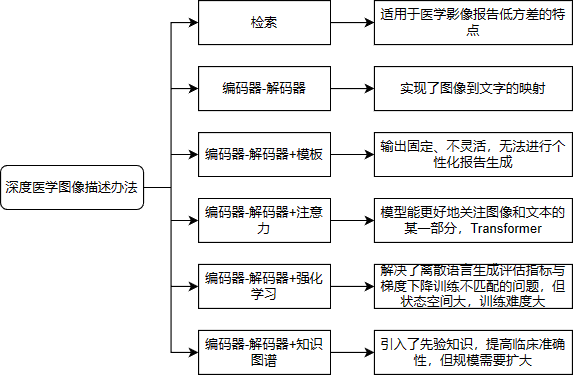
\includegraphics[width=0.95\textwidth]{pic/3.2_structure.png}
       \caption{深度医学图像描述办法}
       \label{Fig_deepmedicalimages}
    \end{figure}

    深度医学图像描述评价指标:主要来自NLP领域。在绝大多数目前的医学图像描述论文中,一定会给出BLEU得分,而ROUGE、METEOR和CIDEr得分会视情况给出部分或全部,其他评价指标虽然理论上可用,但在实际实验中较少使用。

    \section{技术类}
    \subsection{2023年3月 从人脑活动中利用隐式扩散模型进行高分辨率图像重建\cite{takagi2023high}}
    \noindent标题:High-resolution image reconstruction with latent diffusion models from human brain activity\\
    项目主页:\url{https://sites.google.com/view/stablediffusion-with-brain/}\\

    \noindent\textbf{(1).论文试图解决什么问题?}
    \setlength{\parindent}{5ex}

    从人脑活动的fMRI影像中,使用隐式扩散模型方法,重建出受试者看到的视觉影像。

    \noindent\textbf{(2).这是否是一个新的问题}

    从fMRI进行视觉图像重建并不是一个新的问题。但是使用扩散模型进行视觉图像重建是一个新颖的课题。该文章是第一个在该领域使用latent diffusion model的工作。

    \noindent\textbf{(3).这篇文章要验证一个什么科学假设?}

    使用隐式扩散模型重建视觉图像、编码分析和解码分析。并且从神经学的角度,即初级视皮层和高级视皮层的视觉编码功能进行了分析。

    \noindent\textbf{(4).有哪些相关研究?如何归类?谁是这一领域值得关注的研究员?}

    相关工作包括从fMRI中的视觉图像重建和从神经科学角度出发的编码模型。

    本文两位作者均来自大阪大学

    \noindent\textbf{(5).论文中提到的解决方案之关键是什么?}

    LDM和CLIP

    解码过程(从fMRI中重建像):$i.$从初级视皮层的fMRI信号$X$中预测隐式表达$z$,$z$再经由自动编码器的解码模块处理生成一个粗略解码的图像$X_z$。$ii.$ $X_z$经由自动编码器的编码模块处理,然后通过扩散过程添加噪声。$iii.$从高级视皮层的fMRI信号中解码出隐式文本表示$c$,$c$和粗略加入了噪声的隐式表达$Z_T$共同作为去噪的U-Net网络的输入,生成$z_c$。$z_c$输入到自动编码器的解码模块后输出最终的重建图像$X_{zc}$。

    编码过程(全脑体素级建模):$i.$建立线性模型从隐式扩散模型的三个表达$z$,$c$和$z_c$中独自预测体素行为。$ii.$将$z_c$和$z$合并到一个单独的模型中。$iii.$探究迭代去噪过程中$z_c$的变化。$iv.$从U-Net网络的不同层中提取特征。

    其结构见图\ref{overview_cvpr2023}所示。

    \begin{figure}[ptbp]
        \centering
        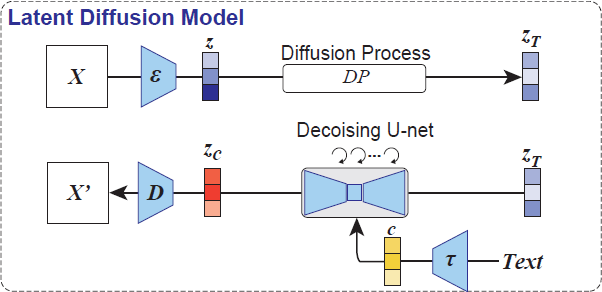
\includegraphics[width=0.95\textwidth]{pic/4.1_latent diffusion model.png}
        \centering
        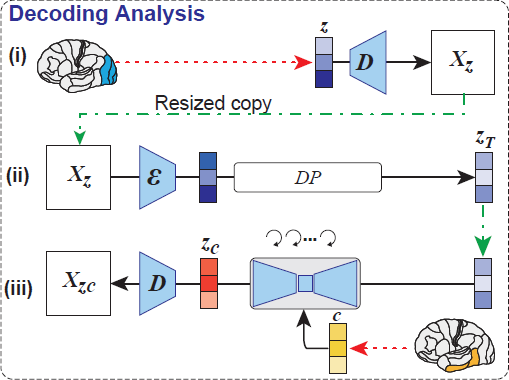
\includegraphics[width=0.95\textwidth]{pic/4.1_decoding analysis.png}
        \centering
        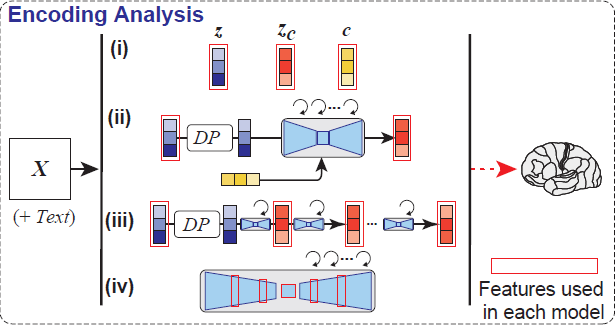
\includegraphics[width=0.95\textwidth]{pic/4.1_encoding analysis.png}
        \caption{Overview of CVPR 2023's work}
        \label{overview_cvpr2023}
    \end{figure}

    \noindent\textbf{(6).论文中的实验是如何设计的?}\\
    最主要的成果展示均来自4名受试者。\\
    \textbf{I.}在解码实验中,

    \textcircled{1}消融实验:\\
    仅使用$z$,重建图像与原始图像在视觉上一致,但不能捕获语义\\
    仅使用$c$,重建图像与原始图像的语义基本一致,但是视觉上不太一致\\
    仅使用$z_c$,重建图像与原始图像的语义和视觉效果均一致

    \textcircled{2}定量实验:使用PSMs(perceptual similarity metrics感知相似度指标)指标定量分析重建图像和原始图像的识别准确度

    \textbf{II.}在编码实验中,

    \textcircled{1}隐式表示间的比较:\\
    $z$,原始图像的隐式表示。在初级视皮层(后部)和高级视皮层(前部)上具有高预测性能。\\
    $c$,图像文本标注的隐式表示。在高级视皮层上具有最高的预测性能。\\
    $z_c$,经过带有$c$的交叉注意力的反扩散过程后,$z$的添加噪声的隐式表示。在初级视皮层上表现出高预测性能。

    \textcircled{2}不同噪声级的比较:\\
    这里所说的噪声是指主要物体的背景复杂度,噪声越低代表物体和背景越容易分离。\\
    噪声较少时,$z$比$z_c$更好地预测了整个皮层的体素活动\\
    噪声较多时,$z_c$比$z$的预测性能更好,图像的语义信息越来越重要

    \textcircled{3}不同扩散阶段的比较:\\
    研究迭代去噪过程中,已添加噪声的潜在表示的改变。去噪过程的早期阶段,$z$主导fMRI图像预测;去噪过程的中期,$z_c$主导了预测。

    \textcircled{4}不同U-Net层的比较:\\
    去噪过程的早期阶段,U-Net的瓶颈层(bottleneck)有最高的预测性能;在后期阶段,U-Net的浅层预测初级视皮层,瓶颈层转向预测高级视皮层。

    \noindent\textbf{(7).用于定量评估的数据集是什么?代码有没有开源?}

    数据集:Natural Scenes Dataset\cite{Allen2022}(\url{http://naturalscenesdataset.org})

    该数据集中受试者所观看的图片-文本信息数据集:MS COCO

    项目代码:\url{https://github.com/yu-takagi/StableDiffusionReconstruction}

    说明:\url{https://sites.google.com/view/stablediffusion-with-brain/faq_en}

    \noindent\textbf{(8).论文中的实验及结果有没有很好地支撑需要验证的科学假设?}

    低层次视觉外观(low-level visual appearance)对应物品的形态对应z对应U-Net网络的前几层对应初级视皮层、高层次语义内容(high-level semantic content)对应物品的抽象语义对应c对应U-Net的瓶颈层对应高级视皮层。

    \noindent\textbf{(9).这篇论文到底有什么贡献?}

    将Latent Diffusion Model用在了大脑视觉场景中,并尝试从神经科学角度对实验中现象进行解释。

    作者自己写的贡献详细看该工作主页。

    \noindent\textbf{(10).下一步呢?有什么工作可以继续深入?}

    没有做生物学上的实验,所以本文从神经生物学提出的对模型实验结果的解释,仅仅只是研究者的“先验思想-初级视皮层解码图像结构,高级视皮层解码语义信息”,并不能作为生命科学的依据。用到的神经学知识不丰富,也不精细。

    做做zero-shot:DALL·E 2\cite{ramesh2022hierarchical}就是zero-shot的生成模型

    这里的视皮层信号是受试者看到的,可以迁移到听到的、想象的、梦境的么。

    人脑的思考个体间差异化很大,跨受试者的迁移模型是一个不错的研究方向。

    \subsection{2022年4月 OpenAI公司提出的基于CLIP模型改进的DALL·E 2模型\cite{ramesh2022hierarchical}}
    \noindent标题:Hierarchical Text-Conditional Image Generation with CLIP Latents\\
    项目主页:\url{https://openai.com/dall-e-2}

    \noindent\textbf{(1).论文试图解决什么问题?}

    从用户提供的文本描述中,生成高质量的图像。

    \noindent\textbf{(2).这是否是一个新的问题}

    在扩散模型流行以前,最流行的模型是GAN。encoder:将图像编码成特征;decoder:从特征重建出图像。

    \noindent\textbf{(3).这篇文章要验证一个什么科学假设?}

    图像生成的多样性,以及贴近文本含义的保真度。

    \noindent\textbf{(4).有哪些相关研究?如何归类?谁是这一领域值得关注的研究员?}

    属于AIGC(AI-Generated Content)范畴下的艺术性的大模型工作。AIGC下的工作值得关注的领域有GAN、VAE、Diffusion Model等。

    论文研究者全部来自OpenAI。

    \noindent\textbf{(5).论文中提到的解决方案之关键是什么?}
    \begin{figure}[ptbp]
        \centering
        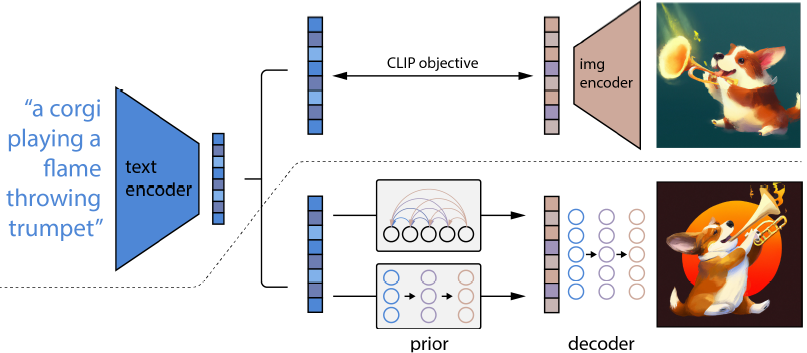
\includegraphics[width=0.95\textwidth]{pic/4.2_unCLIP.png}
        \caption{Overview of DALL E2}
        \label{overview_dalle2}
    \end{figure}

    两个步骤:prior从文本描述生成CLIP的图像嵌入,扩散模型的decoder则以该图像嵌入为条件来生成图像。该图像嵌入是显示生成的

    图\ref{overview_dalle2}的上半是CLIP,下半是DALL·E2。训练prior的时候用CLIP img encoder得到的图像特征作为ground truth做监督,即用文本特征去预测该图像特征。推理阶段,得到图像特征后,用扩散模型的decoder去生成图像。


    \noindent\textbf{(6).论文中的实验是如何设计的?}

    比较自回归先验和扩散先验

    \noindent\textbf{(7).用于定量评估的数据集是什么?代码有没有开源?}

    代码没有开源

    \noindent\textbf{(8).论文中的实验及结果有没有很好地支撑需要验证的科学假设?}

    其工程挑战大于科学意义

    \noindent\textbf{(9).这篇论文到底有什么贡献?}

    人工智能生成的艺术性和大模型的工程处理。

    \noindent\textbf{(10).下一步呢?有什么工作可以继续深入?}

    其生成效果的震撼艺术效果,最直接的影响因素是超大规模的模型训练参数。

    \subsection{2023年5月 MindEye用对比学习和扩散先验来从fMRI中重建视觉图像\cite{Scotti2023ReconstructingTM}}
    \noindent标题:Reconstructing the Mind’s Eye: fMRI-to-Image with Contrastive Learning and Diffusion Priors\\
    项目主页:\url{https://medarc-ai.github.io/mindeye/}

    \noindent\textbf{(1).论文试图解决什么问题?}

    从fMRI影像中重建受试者所看见的视觉图像.

    \noindent\textbf{(2).这是否是一个新的问题}

    该工作在2023CVPRTakagi和Nishimoto\cite{takagi2023high}以及Brain-Diffuser\cite{ozcelik2023natural}的工作之后。

    \noindent\textbf{(3).这篇文章要验证一个什么科学假设?}

    扩散先验技术用到fMRI重建视觉影像任务中,可以增加生成效果和检索性能。

    \noindent\textbf{(4).有哪些相关研究?如何归类?谁是这一领域值得关注的研究员?}

    该文章引用了2023CVPR的Takagi和Nishimoto\cite{takagi2023high}的文章。本文没有涉及到任务有关神经科学与可解释性的内容。

    MindEye的主要作者来自普林斯顿神经科学研究中心和药物AI研究中心

    \noindent\textbf{(5).论文中提到的解决方案之关键是什么?}

     \begin{figure}[ptbp]
        \centering
        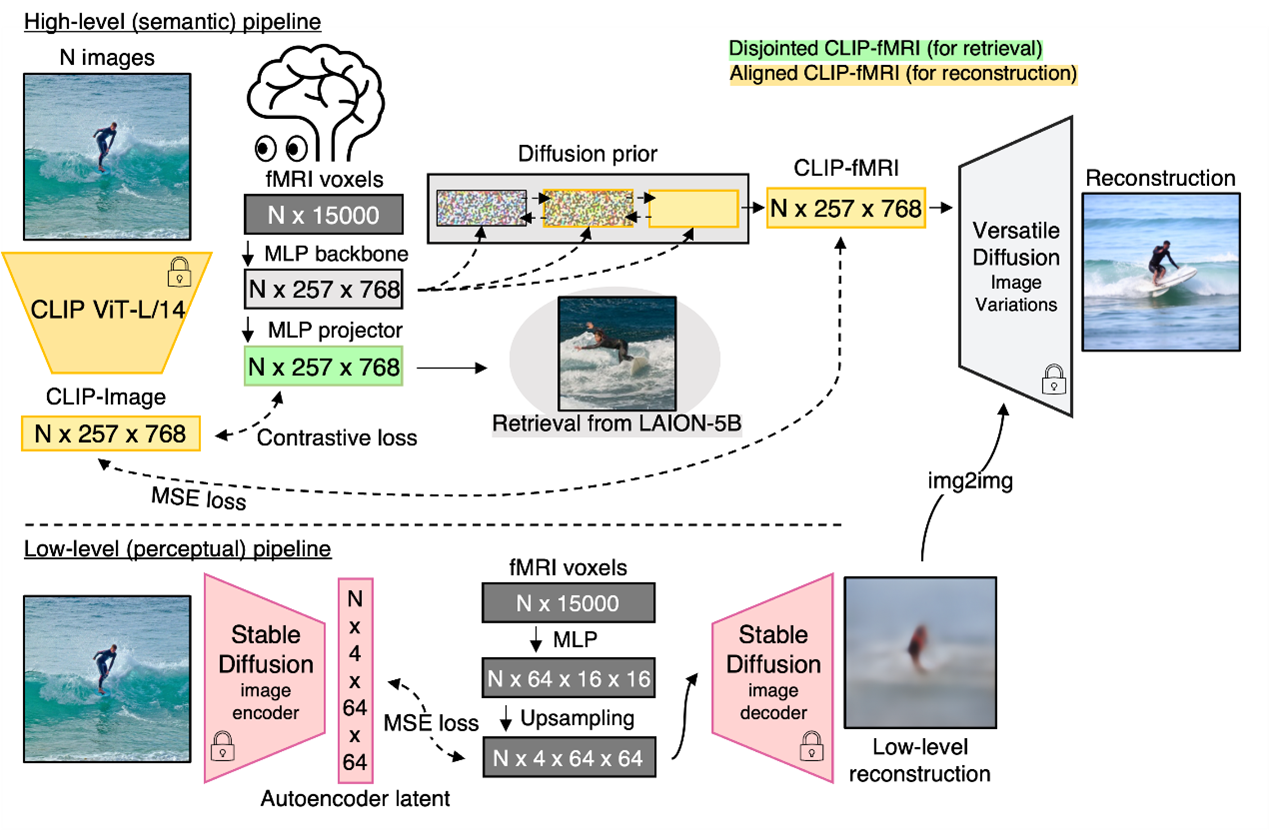
\includegraphics[width=0.95\textwidth]{pic/4.3_mindeye overrall.png}
        \caption{Overview of MindEye}
        \label{overview_mindeye}
    \end{figure}

    MindEye架构如图\ref{overview_mindeye}所示。

    高级语义通道:将fMRI体素映射到CLIP-ViT-L/14的图像空间,用于图像重建和检索任务。对比学习:CLIP是一种跨模态的对比学习方法,MindEye将fMRI作为附加模态添加到预训练的CLIP模型的嵌入空间中。扩散先验:受DALL-E2启发,使用扩散先验来将CLIP文本嵌入映射到CLIP图像空间,其参考的DALL-E2代码链接为https://github.com/lucidrains/DALLE2-pytorch。

    初级感知通道:将fMRI体素映射到stable diffusion的VAE的图像嵌入空间。该通道的输出反馈给VAE的解码器,产出缺失了高级语义内容的模糊图像重建,然后用img2img对重建效果进行提升。

    \noindent\textbf{(6).论文中的实验是如何设计的?}\\
    检索:给定同类候选图像池,基于大脑活动在CLIP空间中找到最相似的一张图像。\\
    重建:从fMRI体素重建出视觉图像。MindEye的扩散先验输出于CLIP-fMRI嵌入是对其的,所以用于重建的扩散模型可以有多种选择,文中使用了Versatile Diffusion、Stable Diffusion和Lafite,其中Versatile Diffusion重建效果最好。\\
    消融:

    对网络架构的消融:对ResBlocks和Skip这两个模块分别进行消融,探究不同架构下检索准确率的变化

    对训练策略的消融:改变损失函数和数据增强策略,探究检索性能的变化。

    对重建策略的消融:主要目的是证明扩散先验的有效性。

    \noindent\textbf{(7).用于定量评估的数据集是什么?代码有没有开源?}

    数据集:自然场景数据集(NSD)\cite{Allen2022}、LATION-5B(\url{https://laion.ai/blog/laion-5b/})

    开源代码:\url{https://github.com/MedARC-AI/fMRI-reconstruction-NSD}

    \noindent\textbf{(8).论文中的实验及结果有没有很好地支撑需要验证的科学假设?}

    实验的种类非常充分,但不清楚每轮实验的时间。

    \noindent\textbf{(9).这篇论文到底有什么贡献?}

    首先是fMRI到视觉图像的二维重建和检索工作,然后在图像生成过程中运用了DALL-E2的扩散先验技术。

    \noindent\textbf{(10).下一步呢?有什么工作可以继续深入?}

    三维,NeRF,渲染出来。(可行性如何)

    反事实推理。(给fMRI体素做脑区mask,然后再重建出来,做可解释性)

    两种mask:人看到的图片有遮挡,不影响人类的视觉语义;机器读取的图片有遮挡,会影响其算法性能。首先对机器识别分割模型做热力图,把对识别最关键的区域给mask起来,然后再分别给机器和人类观看。然后根据人脑fMRI来重建影响,看下重建出来的结果是否是完整的。

    \subsection{2023年1月 Brain-Diffuser利用潜在扩散从fMRI重建自然场景\cite{ozcelik2023natural}}
    \noindent标题:Natural scene reconstruction from fMRI signals using generative latent diffusion

    \noindent\textbf{(1).论文试图解决什么问题?}

    基于fMRI信号重建视觉感知的自然图像。

    \noindent\textbf{(2).这是否是一个新的问题}

    该文章在2023CVPR的Takagi和Nishimoto\cite{takagi2023high}的论文之后,在MindEye\cite{Scotti2023ReconstructingTM}工作之前。

    \noindent\textbf{(3).这篇文章要验证一个什么科学假设?}

    技术上,尽可能提高从fMRI体素中重建视觉图像的质量。科学上,研究大脑不同区域与VDVAE、CLIP-Vision、CLIP-Text三个模块直接的关系、研究大脑不同区域各自最敏感的视觉刺激。

    \noindent\textbf{(4).有哪些相关研究?如何归类?谁是这一领域值得关注的研究员?}

    本文也引用了2023年CVPR的Takagi和Nishimoto的论文。

    Brain-Diffuser的作者向MindEye的作者提供了代码和专业知识。

    Brain-Diffuser的作者来自法国图卢兹大学。

    \noindent\textbf{(5).论文中提到的解决方案之关键是什么?}

    两个阶段:第一个阶段(初阶重建)使用VDVAE(Very Deep Variational Auto Encoder);第二个阶段(最终重建)训练了两个回归模型,一个从fMRI映射到CLIP视觉特征、一个从fMRI映射到CLIP文本特征。最终使用预训练的Versatile Diffusion模型来完成图像重建。

    初阶重建/第一阶段:VDVAE(一个分层的VAE模型)能重建出VAE无法生成的复杂自然图像。如下图,该过程的训练阶段,每张图像经由VDVAE编码器处理成一个隐向量;该过程的测试阶,每个隐向量经由VDVAE解码器生成64×64的图像,该低水平的重建图像用作第二阶段的扩散模型的initial guess。该阶段见图\ref{brain-diffuser first stage}。

    \begin{figure}[htbp]
        \centering
        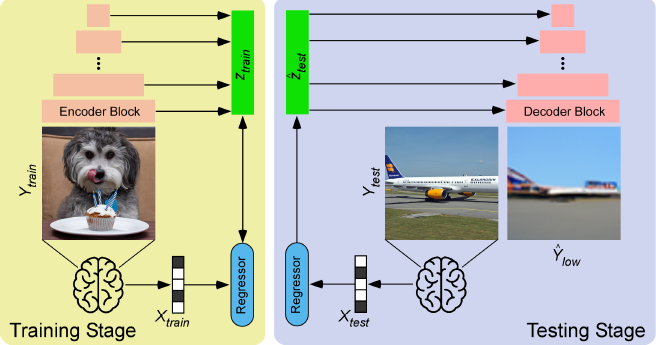
\includegraphics[width=0.95\textwidth]{pic/4.4_first stage.png}
        \caption{Brain-Diffuser first stage}
        \label{brain-diffuser first stage}
    \end{figure}

    最终重建/第二阶段:Versatile Diffusion也是一种latent diffusion model,用来生成VDVAE无法生成的高级特征。该阶段的训练过程两个回归模型:fMRI到CLIP-Vision特征的模型,有257个长度为768的embedding,一个embedding表示该图像的类别相关的信息,其余256个embedding表征从图像中截取的patches;fMRI到CLIP-Text特征的模型,从该图像在COCO的文本描述种提取77个768维的embedding。该阶段的测试过程使用了latent diffusion model的image-to-image pipeline,首先将已经用VDVAE重建过的图像从64×64上采样到512×512,再用AutoKL编码器进行编码,并在前向扩散过程中往隐向量中添加噪音,然后是去噪过程,去噪过程中用的是Versatile Diffusion的双引导扩散pipeline,所谓的双引导是说去噪过程中用CLIP-Vision特征和CLIP-Text特征同时加以条件约束,最终由AutoKL的解码器来生成512×512重建结果。该阶段见图\ref{brain-diffuser second stage}。

    \begin{figure}[htbp]
        \centering
        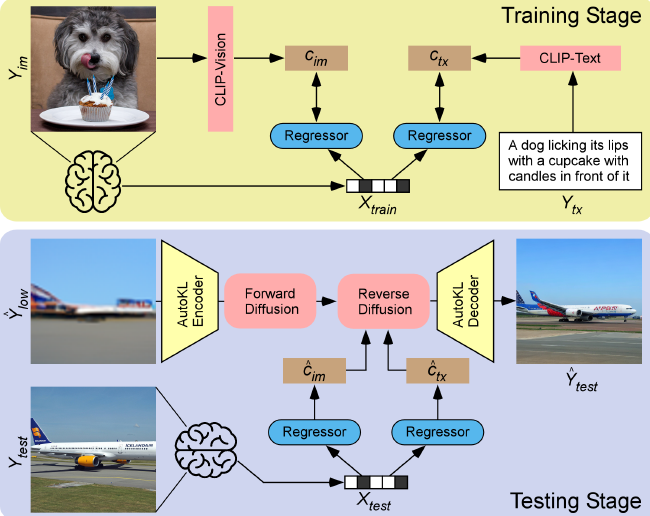
\includegraphics[width=0.8\textwidth]{pic/4.4_second stage.png}
        \caption{Brain-Diffuser second stage}
        \label{brain-diffuser second stage}
    \end{figure}

    \noindent\textbf{(6).论文中的实验是如何设计的?}

    图像重建的对比实验:第一个使用NSD数据集进行重建研究的Mind Reader(Lin, NeurIPS, 2022),用StyleGAN进行图像生成;2023CVPR的Takagi和Nishimoto使用NSD数据集进行重建研究,第一个使用latent diffusion model的;2023年MIDL(Medical Imaging with Deep Learning)上的Cortex2Image使用了在ImageNet上训练的Instance-Conditional GAN模型。

    fMRI重建的定量指标:低阶有PixCorr、SSIM、AlexNet;高阶有Inception、CLIP、EffNet-B、SwAV。每个参数的具体含义在论文中有所交代。

    消融实验:分别去掉VDVAE、CLIP-Vision、CLIP-Text。三种变体和原架构的定性和定量结果均有。可解释性实验:目的是研究大脑区域和模型的组成部分VDVAE、CLIP-VIsion、CLIP-Text之间的联系,方法是对回归权重进行region-of-interest(ROI)分析。结果是VDVAE特征与初级区域(V1~V4区域)关联紧密,CLIP特征则关联到特定类别的高级大脑区域(Words、Faces、Bodies、Places)。

    对大脑特定region-of-interest(ROI)区域的功能研究:目的是可视化大脑特定区域的最佳刺激,这里所说的最佳刺激是指最能激活该特定区域、而尽量不激活其他区域的图像。对V1、V2、V3、V4、Face-ROI、Word-ROI、Place-ROI、Body-ROI这8个ROI进行了分析。

    \noindent\textbf{(7).用于定量评估的数据集是什么?代码有没有开源?}

    数据集:自然场景数据集Natural Scenes Datasets\cite{Allen2022}

    开源代码:\url{https://github.com/ozcelikfu/brain-diffuser}

    \noindent\textbf{(8).论文中的实验及结果有没有很好地支撑需要验证的科学假设?}

    图像重建所提供的baseline值得后续关注。

    另外其两个有关神经科学可解释性的实验方法和定量指标也很值得关注。

    \noindent\textbf{(9).这篇论文到底有什么贡献?}

    论文结构是非常规范的,阅读起来比较自然。首先是双阶段(先生成粗略底图再用扩散模型生成最终结果)和有引导(CLIP的图像特征和文本特征)的扩散模型的思路是非常自然且清晰的。然后是可解释性实验部分具有很大的借鉴意义。

    \noindent\textbf{(10).下一步呢?有什么工作可以继续深入?}

    人脑作为编码器添加到整个算法pipeline中:人类阅读某段文本,想象出画面,然后由机器进行解码。即对想象视觉的可解释性研究。

    视觉的深度信息在哪里?应该数据集中是有的吧

    \subsection{2022年4月 基于非侵入人脑记录的连续语言的语义重建\cite{tang2023}}
    \noindent标题:Semantic reconstruction of continuous language from non-invasive brain recordings
    项目主页:\url{https://www.nature.com/articles/s41593-023-01304-9}

    \noindent\textbf{(1).论文试图解决什么问题?}

    目的是建立一个可以从fMRI语义皮层影像中重建出连续语言的非侵入性语义解码器。

    \noindent\textbf{(2).这是否是一个新的问题}

    从fMRI来生成完整的英语句子,是本文比较突出的一个工作创新。

    \noindent\textbf{(3).这篇文章要验证一个什么科学假设?}

    除了针对大脑的编码解码外,还训练了一个序列预测的GPT模型,该GPT模型给大脑编码解码提供了限定范围。

    \noindent\textbf{(4).有哪些相关研究?如何归类?谁是这一领域值得关注的研究员?}

    德克萨斯州大学奥斯丁分校计算机科学系和神经科学系。

    \noindent\textbf{(5).论文中提到的解决方案之关键是什么?}

    \textbf{a.}三名受试者听了16小时的叙述性故事,记录BOLD fMRI反应,从而构建每个受试者的编码模型(encoding model),以预测词语的语义特征刺激时的大脑反应。\textbf{b.}解码器维护一个候选单词序列的集合以从新的大脑记录中重建出语言。当检测到新单词的时候,语言模型(一个微调过的GPT网络)为每个序列生成一句连续的语句,而编码模型则对每个连续语句与已记录的大脑反应之间的似然进行评分,最为相似的连续语句将被留存。\textbf{c.}解码器(decoders)用来对受试者在聆听一段训练集中从未听过的测试语音时单次实验中大脑响应的记录进行评估。这三个步骤见图\ref{step a2c}。

    \begin{figure}[htbp]
        \centering
        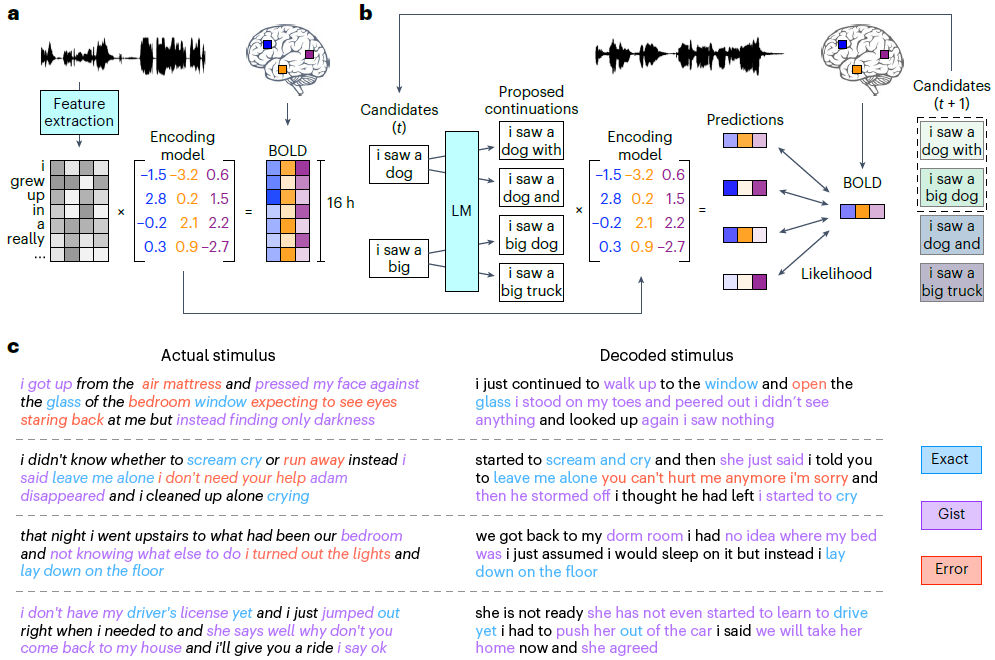
\includegraphics[width=0.95\textwidth]{pic/4.5_step a2c}
        \caption{步骤a到c}
        \label{step a2c}
    \end{figure}

    \noindent\textbf{(6).论文中的实验是如何设计的?}

    将语言处理过程中活跃的脑皮层分成三个区域:speech network、parietal-temporal-occipital association region顶骨颞骨枕骨关联区、prefrontal region。解码实验分别在每个半球的每个区域上进行。

    跨模态解码:听语音讲故事(扬声器刺激)、想象讲5个1分钟的故事、观看4部无声短片、扬声器刺激更换男音或者女音。

    分析解码错误的来源:分析了训练数据集大小对解码性能的影响、测试集的低信噪比(signal-to-noise ratio, SNR)也可能限制了能被解码的信息的总量、不同的扫描仪也会影响解码器

    \noindent\textbf{(7).用于定量评估的数据集是什么?代码有没有开源?}

    数据集:来自OpenNeuro的$ds003020$和$ds004510$。

    开源代码:\url{https://github.com/HuthLab/semantic-decoding}

    \noindent\textbf{(8).论文中的实验及结果有没有很好地支撑需要验证的科学假设?}

    实验部分文字内容太多。

    \noindent\textbf{(9).这篇论文到底有什么贡献?}

    \noindent\textbf{(10).下一步呢?有什么工作可以继续深入?}

    神经科学和计算机科学的工作均非常深入。

    抓住图像、自然语言这样的多模态信息。

    \subsection{2023年8月 Algonauts2023挑战赛第一名解决方案\cite{yang2023memory}}
    \noindent标题:Memory Encoding Model\\
    项目主页:\url{https://huzeyann.github.io/mem}

    \noindent\textbf{(1).论文试图解决什么问题?}

    Algonauts 2023挑战赛的目标是预测受试者观看复杂自然视觉场景时所被记录的大脑反应。本文使用记忆过程(memory process)来增强大脑编码模型(brain encoding model)。

    \noindent\textbf{(2).这是否是一个新的问题}

    是从fMRI重建出受试者看到的视觉影像的逆问题。比较典型的神经科学对机器学习的启发。

    \noindent\textbf{(3).这篇文章要验证一个什么科学假设?}

    基于周期性延迟反应(periodic delayed response)和海马体尾部活动(hippocampus tail activity)的实验观察而提出了“记忆过程(memory process)影响大脑编码模型(brain encoding model)”的理论。

    \noindent\textbf{(4).有哪些相关研究?如何归类?谁是这一领域值得关注的研究员?}

    绘制视皮层的工具:{\sffamily{pycortex}}。

    该工作的三名作者均来自宾夕法尼亚大学。

    \noindent\textbf{(5).论文中提到的解决方案之关键是什么?}

    视觉刺激+记忆信息+行为反应,共同构成了决定当前大脑全皮层活动的输入。如果仅仅关注当前受试者所看到的视觉刺激,那么仅能预测出初级视皮层的活动。行为反应则包括按下按钮和凝视。

    RetinaMapper和LayerSelector两个模块专注于复制(replicate)视网膜拓扑映射(retinotopy\cite{Engel1997RetinotopicOI})。

    预实验:在NSD数据集上发现,视觉和非视觉大脑的活动与前第6个或者第7个看到的图像相关,而非是刚才的1~2张图像。在NSD数据集上的8个受试者的数据中,均观察到了该现象;海马体尾部预测的反应与这个周期性是相符合的,但是海马体头部预测的反应则与之不相符。但是这样的周期律在\textbf{BOLD5000}数据集上没有被发现。因此需要注意,该预实验得到的先验知识来自于NSD数据集,暂且没有神经学自然科学理论的支持。

    \begin{figure}[htbp]
        \centering
        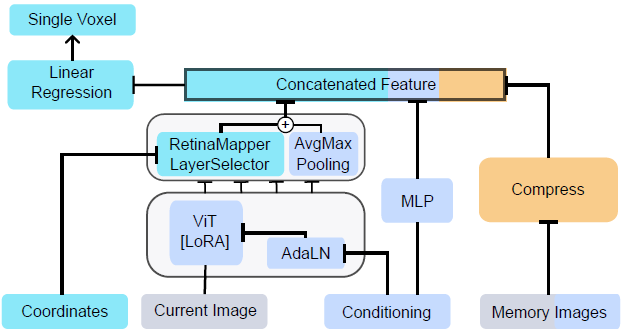
\includegraphics[width=0.95\textwidth]{pic/4.6_memory encoding model}
        \caption{Overview of memory encoding model}
        \label{overview mem}
    \end{figure}

    该模型的结构图见\ref{overview mem}所示。

    RetinaMapper将体素的三维空间坐标转换为图像空间的二维坐标。LayerSelector将体素的三维空间坐标转换为ViT主干层的四维权重。

    提高模型得分的手段:增加了前一帧图像的输入、随机ROI区域组装或者模型蒸馏。

    \noindent\textbf{(6).论文中的实验是如何设计的?}

    指标:噪声上限(noise ceiling)是衡量大脑初级视觉部分数据质量的精准指标。

    \noindent\textbf{(7).用于定量评估的数据集是什么?代码有没有开源?}

    数据集:Algonauts 2023、NSD、BOLD5000

    开源代码:\url{https://github.com/huzeyann/MemoryEncodingModel}

    \noindent\textbf{(8).论文中的实验及结果有没有很好地支撑需要验证的科学假设?}

    该工作经过预实验发现了NSD数据集上的周期性延迟响应(periodic delayed response)的特点,后续的实验证明了这个观察到的现象确实是存在的,但是没有合理的解释。

    \noindent\textbf{(9).这篇论文到底有什么贡献?}

    发现了NSD数据集上的周期性延迟响应(periodic delayed response)

    \noindent\textbf{(10).下一步呢?有什么工作可以继续深入?}

    文中提到的周期性延迟响应(periodic delayed response)是什么机理、什么原因?其他数据集上有类似的结论么?有什么生物学依据么?


    \subsection{2023年8月 Algonauts2023挑战赛第二名解决方案\cite{Adeli2023.08.02.551743}}
    \noindent标题:Predicting brain activity using Transformers

    \noindent\textbf{(1).论文试图解决什么问题?}

    Algonauts 2023挑战赛的目标是预测受试者观看复杂自然视觉场景时所被记录的大脑反应。用Transformer机制(自注意力和交叉注意力self and cross-attention)来学习从自然场景图像特征到大脑反应的映射。

    \noindent\textbf{(2).这是否是一个新的问题}

    是从fMRI重建出受试者看到的视觉影像的逆问题。

    \noindent\textbf{(3).这篇文章要验证一个什么科学假设?}

    使用Transformer的encode-decode方法来完成从自然场景图像预测fMRI的任务。

    \noindent\textbf{(4).有哪些相关研究?如何归类?谁是这一领域值得关注的研究员?}

    该工作的3名作者均来自哥伦比亚大学。

    相关工作:自监督的视觉自注意力模型(Self-supervised Vision Transformers)、编码器-解码器的视觉自注意力模型(Encoder-decoder Vision Transformers)

    \noindent\textbf{(5).论文中提到的解决方案之关键是什么?}

    使用Transformer的encoder-decoder模型来学习从自然场景图像到fMRI的映射。encoder是使用自监督方法(DINOv2)训练的视觉转换器。decoder则用来预测每个兴趣区域(region-of-interest, ROI)中的神经活动。其架构见图\ref{second team architecture}所示。

    \begin{figure}[htbp]
       \centering
       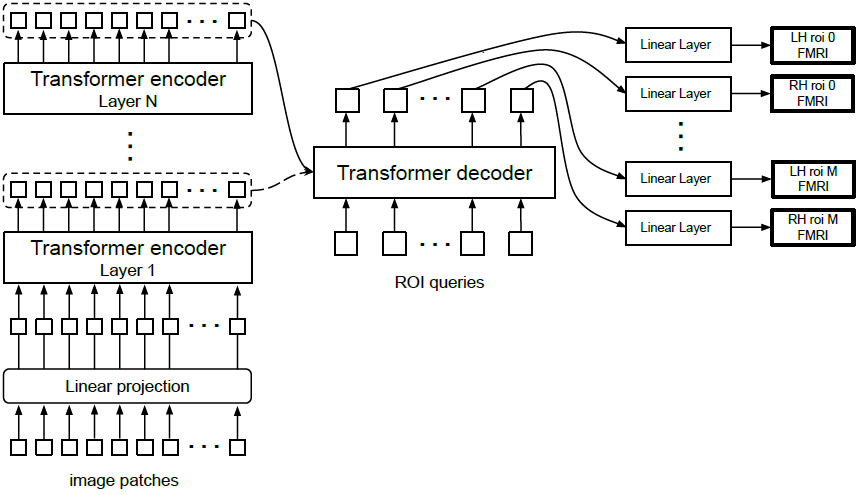
\includegraphics[width=0.95\textwidth]{pic/4.7_model architecture}
       \caption{Model Architecture}
       \label{second team architecture}
    \end{figure}

    \noindent\textbf{(6).论文中的实验是如何设计的?}

    本论文更倾向于是一篇技术报告。

    \noindent\textbf{(7).用于定量评估的数据集是什么?代码有没有开源?}

    数据集:Algonauts2023挑战赛数据集。

    开源代码:https://github.com/Hosseinadeli/algonauts2023\_transformers

    \noindent\textbf{(8).论文中的实验及结果有没有很好地支撑需要验证的科学假设?}

    论文中提供的实验并不充分,且第二名的得分与第一名具有较大差距。

    \noindent\textbf{(9).这篇论文到底有什么贡献?}

    视觉自注意力模型的encoder、decoder方案是一个非常基础且的确实用的思路。

    \noindent\textbf{(10).下一步呢?有什么工作可以继续深入?}

    可以在encoder-decoder的思路上更换模块、拓展任务驱动。

    \subsection{2023年8月 Algonauts2023挑战赛第三名解决方案\cite{nguyen2023algonauts}}
    \noindent标题:THE ALGONAUTS PROJECT 2023 CHALLENGE: UARK-UALBANY TEAM SOLUTION

    \noindent\textbf{(1).论文试图解决什么问题?}

    Alognauts 2023挑战赛的目标是预测受试者观看复杂自然视觉场景时被记录的大脑反应。

    \noindent\textbf{(2).这是否是一个新的问题}

    是从fMRI重建出受试者看到的视觉影像的逆问题。

    \noindent\textbf{(3).这篇文章要验证一个什么科学假设?}

    模型评价指标:平均噪音归一化编码准确度(mean noise-normalized encoding accuracy)

    \noindent\textbf{(4).有哪些相关研究?如何归类?谁是这一领域值得关注的研究员?}

    本文三名作者均来自于阿肯色大学。

    \noindent\textbf{(5).论文中提到的解决方案之关键是什么?}

    针对所有受试者进行统一的预训练。见图\ref{pretrain stage}。
    \begin{figure}[htbp]
        \centering
        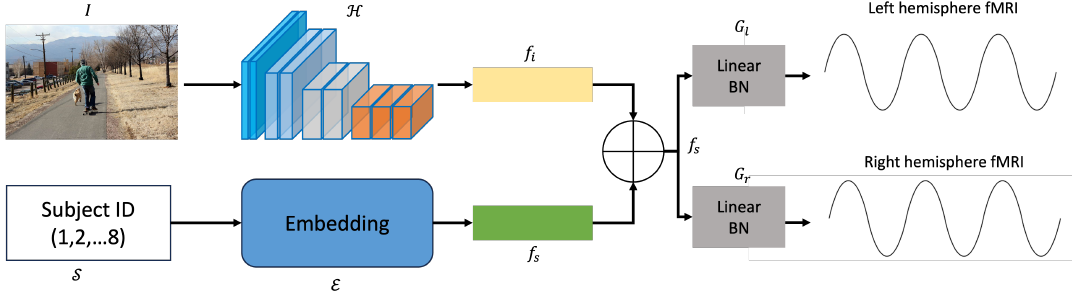
\includegraphics[width=0.95\textwidth]{pic/4.8_pretraining stage}
        \caption{预训练阶段}
        \label{pretrain stage}
    \end{figure}

    针对每个受试者进行各自的微调。见图\ref{fine-tuning stage}。
    \begin{figure}[htbp]
        \centering
        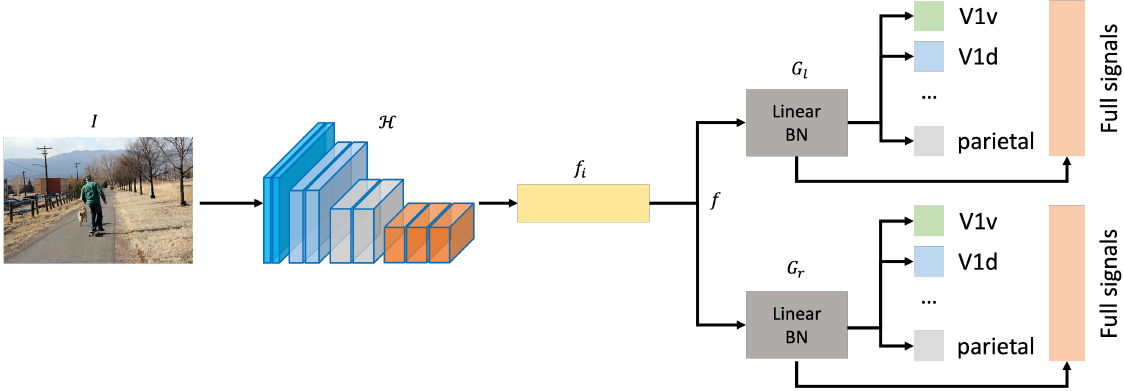
\includegraphics[width=0.95\textwidth]{pic/4.8_fine-tuning stage}
        \caption{微调阶段}
        \label{fine-tuning stage}
    \end{figure}

    \noindent\textbf{(6).论文中的实验是如何设计的?}

    无值得关注处。

    \noindent\textbf{(7).用于定量评估的数据集是什么?代码有没有开源?}

    数据集:Algonauts2023挑战赛数据集。

    开源代码:https://github.com/uark-cviu/Algonauts2023

    \noindent\textbf{(8).论文中的实验及结果有没有很好地支撑需要验证的科学假设?}

    无值得关注处。

    \noindent\textbf{(9).这篇论文到底有什么贡献?}

    预训练+微调(fine-tuning)的方式虽然经典,但是值得借鉴。

    \noindent\textbf{(10).下一步呢?有什么工作可以继续深入?}

    无值得关注处。

    \subsection{2022年NeurIPS Mind Reader从大脑活动重建复杂图像\cite{NEURIPS2022_bee5125b}}
    \noindent标题:{Mind Reader:Reconstructing complex images from brain activities}
    \noindent\textbf{(1).论文试图解决什么问题?}

    从大脑活动的fMRI影像中重建出具有丰富语义信息的自然图片。

    \noindent\textbf{(2).这是否是一个新的问题}

    是第一个从大脑活动重建复杂图像的工作。

    \noindent\textbf{(3).这篇文章要验证一个什么科学假设?}

    跨模态的图像重建问题,以及各个脑区对刺激的不同响应。

    \noindent\textbf{(4).有哪些相关研究?如何归类?谁是这一领域值得关注的研究员?}

    三名来自伯克利大学圣塔芭芭拉的学者,按照文中所说,该问题下这是第一个工作。实验室为DYNAMO,该小组的主页为:\url{https://dynamo.cs.ucsb.edu/publications}。但是在其2023年发表的论文中,目前没有找到与大脑or人眼视觉相关的工作。

    \noindent\textbf{(5).论文中提到的解决方案之关键是什么?}

    开创了两阶段重建的方法:第一阶段训练了两个映射模型$f_{mi}$和$f_{mc}$将fMRI编码到CLIP嵌入空间;第二阶段条件生成器G和对比鉴别器D在$f_{mi}$和$f_{mc}$的前提下微调。本文提出,从头学习大脑编码-译码模型是困难的,因此从预训练的对比模型中获得对齐嵌入(aligned embeddings),以这些嵌入作为生成图像的条件。

    将fMRI信号映射到CLIP空间:训练了两个映射模型,$f_{mi}$和$f_{mc}$,前者为CLIP图像编码器,后者为CLIP文字编码器。

    CLIP嵌入条件下的图像重建:生成模型是Lafite,一个文本到图像的生成模型,它将无条件的StyleGAN应用于基于CLIP文本嵌入的条件图像生成。

     \begin{figure}[htbp]
        \centering
        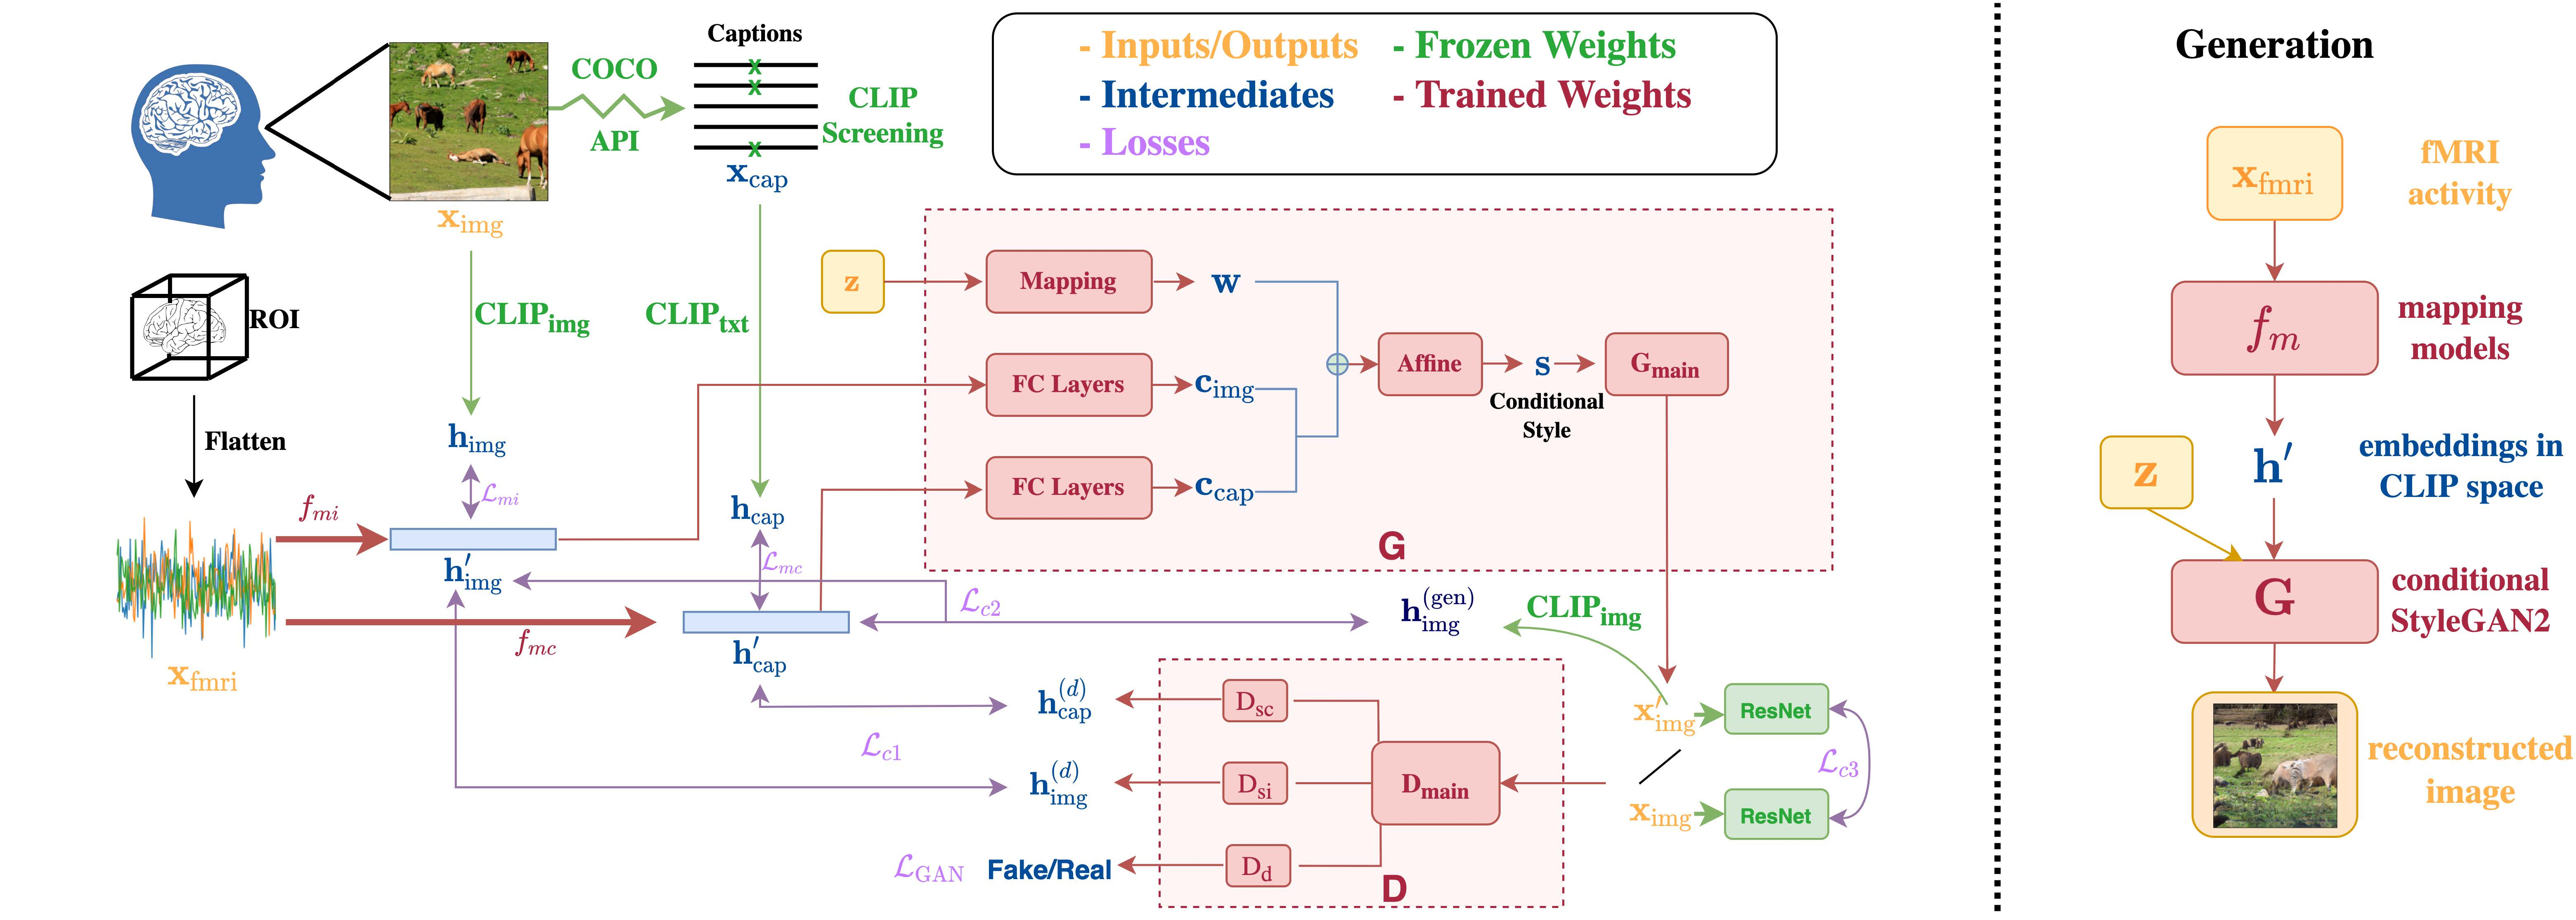
\includegraphics[width=0.95\textwidth]{pic/4.9_pipeline.jpg}
        \caption{模型流水线}
        \label{pipeline}
    \end{figure}

    \noindent\textbf{(6).论文中的实验是如何设计的?}

    限制:由于不同个体之间大脑的编码和感知是不同的,因此本工作专注于从单个受试者的大脑信号中重建其观看的场景。

    将fMRI信号映射到CLIP嵌入:使用两个指标来评价映射模型的性能。第一个指标是生成图像和预训练模型生成器的ground truth之间的Fréchet Inception Distance。第二个指标是图像的retrieval成功率。

    结合神经生物学的为刺激实验:该实验对大脑不同ROI区域中体素的输入fMRI信号施加微刺激,旨在识别单个区域的作用。作者通过该实验发现CLIP embeddings解耦空间(disentangled space)与人脑处理视觉线索的方式非常一致。

    \noindent\textbf{(7).用于定量评估的数据集是什么?代码有没有开源?}

    数据集:Natural scenes dataset\cite{Allen2022}

    开源代码:\url{https://github.com/sklin93/mind-reader}

    \noindent\textbf{(8).论文中的实验及结果有没有很好地支撑需要验证的科学假设?}

    字多图少数据少。该工作将图像重建问题视为信号到信号的转换,并且尝试了类似于DALL-E的架构(不是DALL-E2,DALL-E2用的扩散模型,该文章没有)。

    \noindent\textbf{(9).这篇论文到底有什么贡献?}

    开创了这个方面,但是我觉得自NeurIPS和CVPR之后,再没啥生成框架好用的了,NeurIPS这篇用的GAN,CVPR换成Diffusion Model,其余的CLIP embedding和神经生物学解释基本上都是如出一辙的,cvpr的实验确实更充分些。

    \noindent\textbf{(10).下一步呢?有什么工作可以继续深入?}

    要么联系神经生物学更强, 要么脱离生成式框架。


    \subsection{2023年ICCV Best Paper 向文字到图像的扩散模型中添加条件控制\cite{zhang2023adding}}
    \noindent标题:{Adding Conditional Control to Text-to-Image Diffusion Models}

    \noindent\textbf{(1).论文试图解决什么问题?}

    本文提出了端到端的神经网络架构ControlNet,在微调(finetuning)阶段将空间条件控制(spatial conditioning controls)添加到预训练的文本-图像生成大模型稳定扩散(Stable Diffusion)中,目的是控制图像扩散模型。

    \noindent\textbf{(2).这是否是一个新的问题}

    OpenAI公司的DALLE2模型\cite{ramesh2022hierarchical}也是有条件限制的用于图像生成的扩散模型,其条件来自从用户输入的自然语言中提取的语义信息。而ControlNet所用的条件是基于图形学的,比如Canny边缘检测算法算出来的边缘(Canny edges)、霍夫线条(Hough lines)、用户涂鸦(user scribbles)、人体关键点(human key points)、分割图谱(segmentation maps)、表面形状的法线(shape normal)、深度(depths)、卡通线条(cartoon line drawings)。

    \noindent\textbf{(3).这篇文章要验证一个什么科学假设?}

    在文本生成图像的扩散模型的微调阶段,添加学习得到的图形学监督条件,从而控制生成的图像。

    \noindent\textbf{(4).有哪些相关研究?如何归类?谁是这一领域值得关注的研究员?}

    其所用的图形学条件监督,本质上都是对几何物体(边缘特征、关键点、区域分割、表面法线)的约束。在NeRF Editing相关的工作中,同样有使用sketch类约束的,如Sketch Face Editing等。

    \noindent\textbf{(5).论文中提到的解决方案之关键是什么?}

    \noindent{5.1.ControlNet基本结构}

    图\ref{ControlNet}中所说的neural network block代指若干个神经网络层组织起来的功能块,比如残差块、卷积块、多头注意力块、Transformer块等。将ControlNet添加到神经网络块中,先将原始块的参数集$\Theta$锁住保持不变,将$\Theta$拷贝一份得到$\Theta_c$作用可训练的参数集。可训练的部分有两个输入,一个是原始特征图$x \in \mathbb{R}^{h \times w \times c}$,另一个是条件向量(conditioning vector)$c$。将该模式用在Stable Diffusion中,被锁定的原始参数集$\Theta$就是一个保留了几十亿(billions)张图像的预训练模型。

    图\ref{ControlNet}左侧的被锁定模型记为$\mathcal{F}(x;\Theta)$。图\ref{ControlNet}右侧的可训练拷贝通过零卷积层(zero convolution layers)$\mathcal{Z}(\cdot;\cdot)$连到$\mathcal{F}(x;\Theta)$。$\mathcal{Z}(\cdot;\cdot)$是一个$1\times1$的卷积层,其权重和偏置都初始化为$0$。作者使用了两个零卷积层,独立的训练两个参数集$\Theta_{z1}$和$\Theta_{z2}$,最终的输出为:$y_c=\mathcal{F}(x;\Theta)+\mathcal{Z}(\mathcal{F}(x+\mathcal{Z}(c;\Theta_{z1});\Theta_c);\Theta_{z2})$。从该公式中能够推断出为何作者要将零卷积层的初始化权重和偏置都设为$0$,因为这样在第一轮次的训练中就有$y_c = y$,保留了预训练大模型的性能。

    \begin{figure}[htbp]
        \centering
        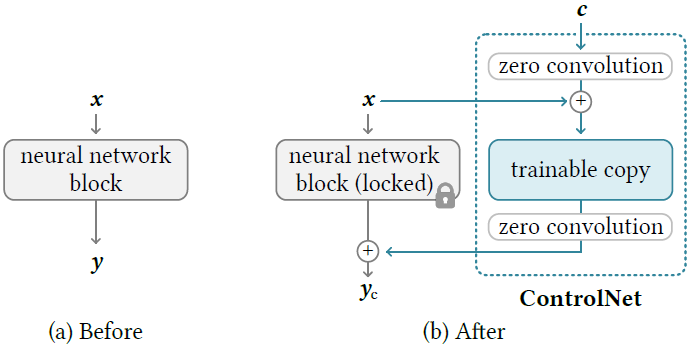
\includegraphics[width=0.95\textwidth]{pic/4.10_ControlNet.png}
        \caption{ControlNet}
        \label{ControlNet}
    \end{figure}

    \noindent{5.2.将ControlNet用到Stable Diffusion中}

    Stable Diffusion本质上是一个U-Net,有一个编码器(encoder)、中间块(middle block)和跳层连接解码器(skip-connected decoder),其中编码器和解码器各自有12个块、中间层仅有一个块,即一共25个块(这里所划分的块就是上文所述的neural network block)。25个块中,8个块是下采样或者上采样卷积层,其余17个块是主块,每个住块包括4个残差层和2个视觉Transformer(Vision, ViT)。每个ViT包含了若干个交叉注意力(cross-attention)和自注意力(self-attention)机制。作者将ControlNet添加到U-Net编码器的每一层(12个)。

    \noindent\textbf{(6).论文中的实验是如何设计的?}

    \noindent{6.1.定性生成结果}

    图\ref{ControlNetResults}的每一列为不同的条件监督,从左到右依次为:Sketch、Normal map、Depth map、Canny edge、M-LSD line、HED edge、ADE20kseg、Human pose。第一行是输入的条件,其余行都是模型的输出。

    \begin{figure}[htbp]
        \centering
        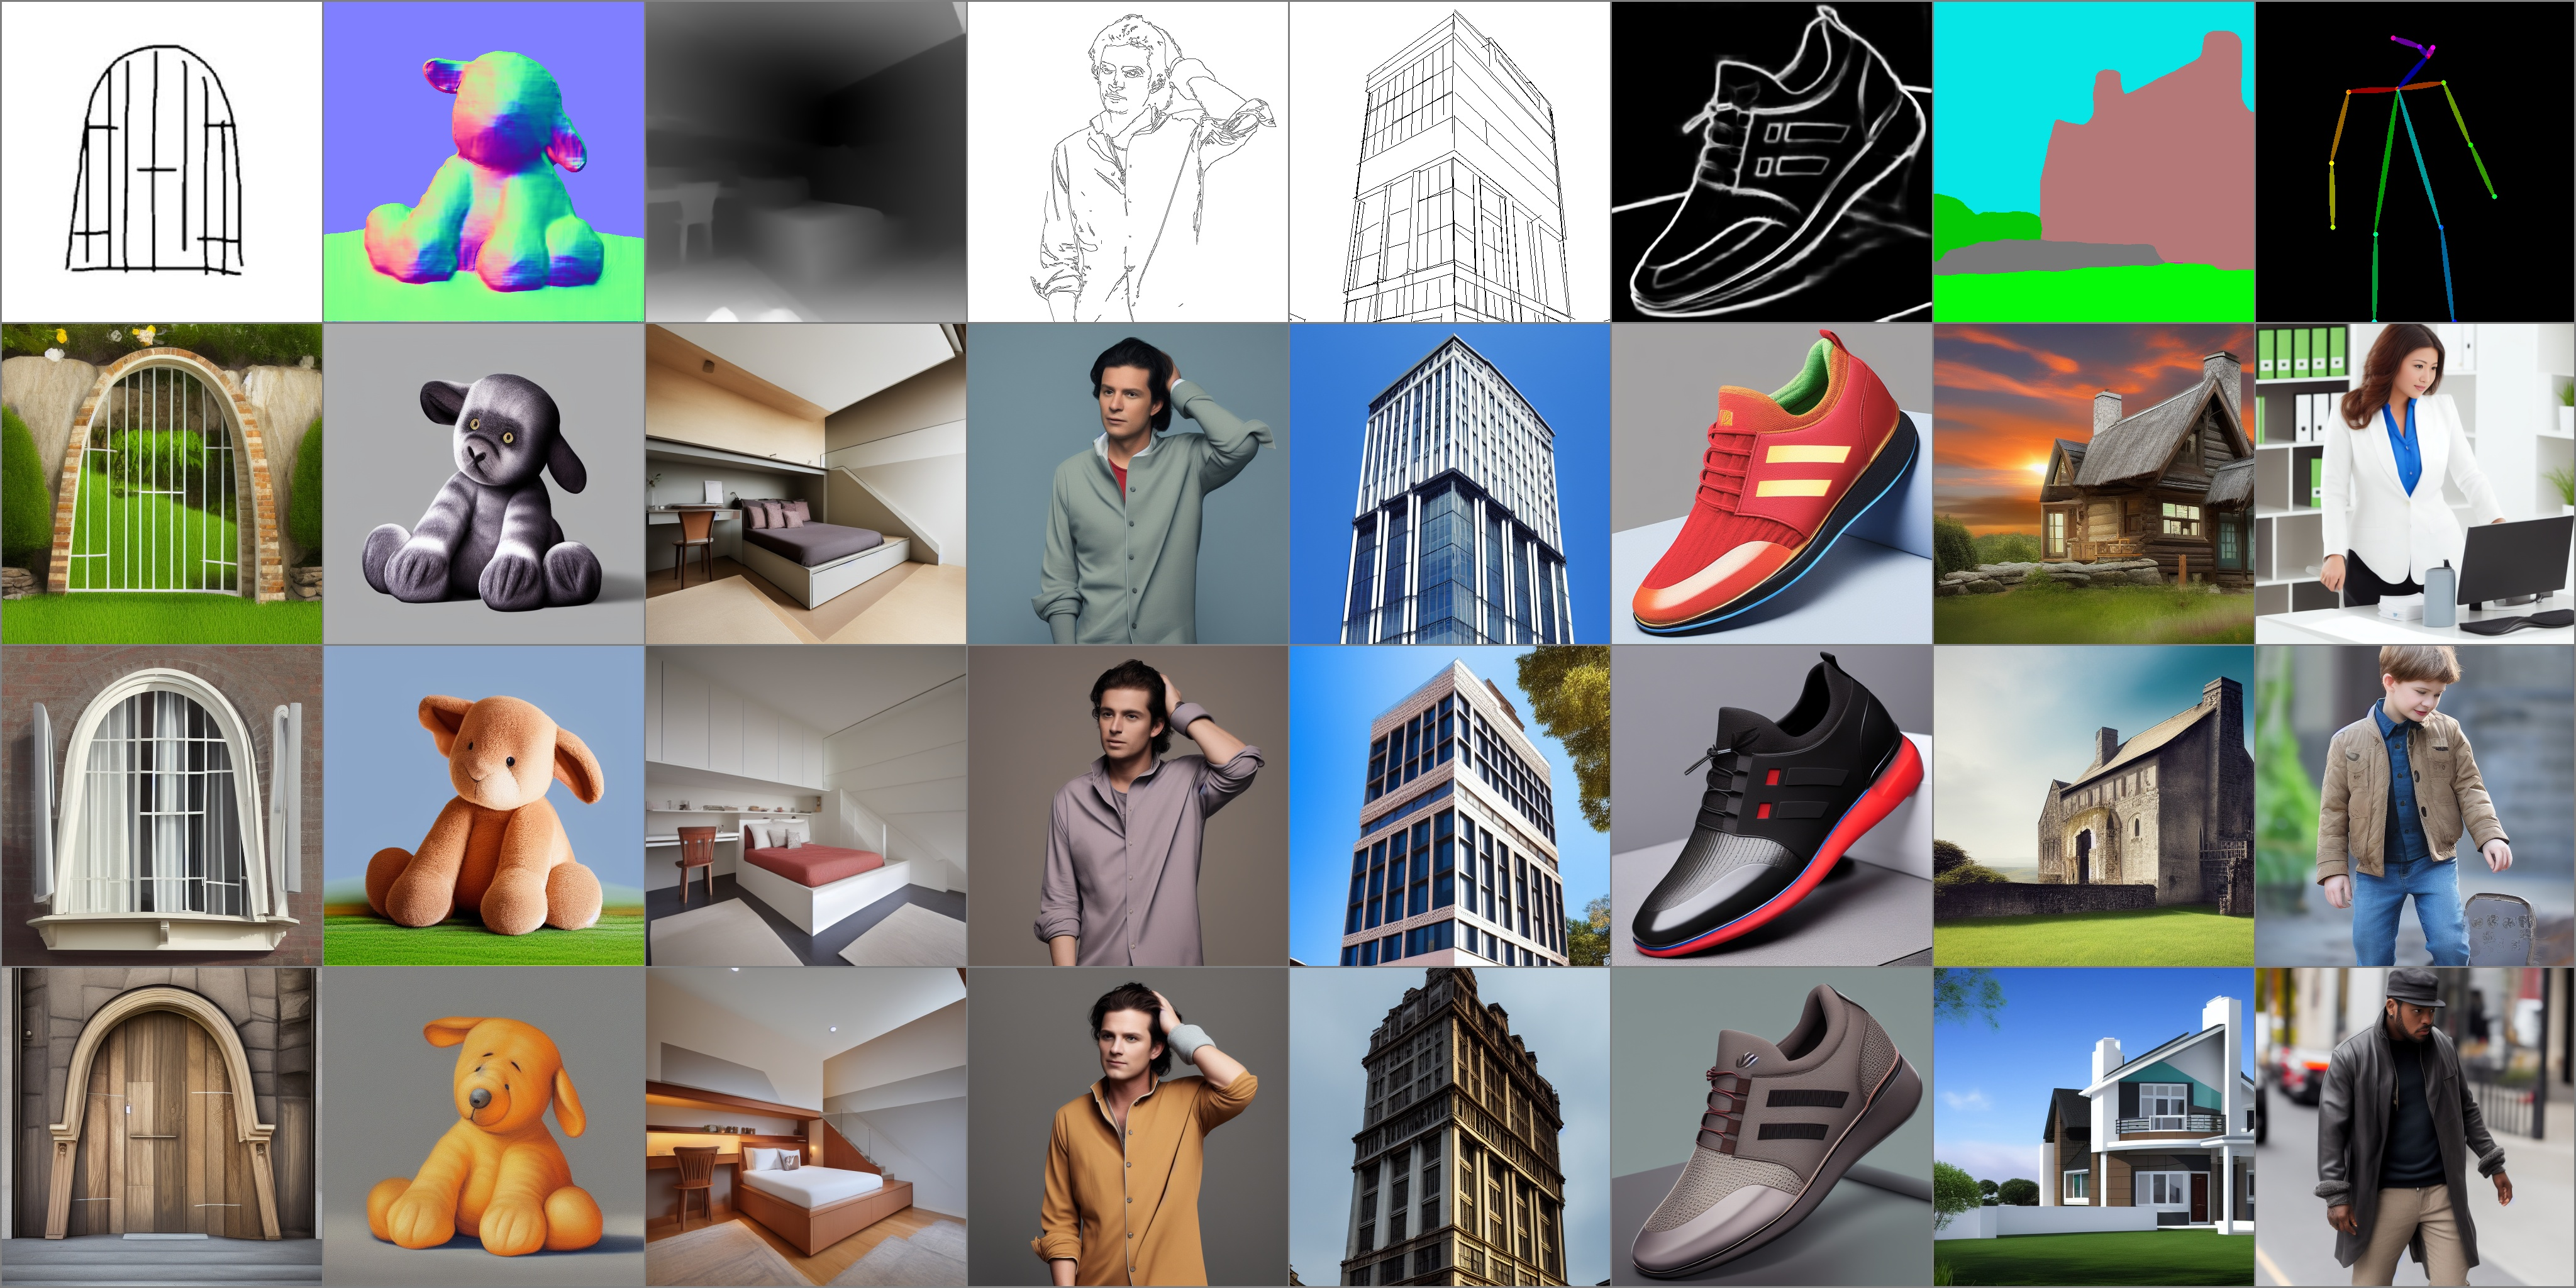
\includegraphics[width=0.95\textwidth]{pic/4.10_ControlNetResults.jpg}
        \caption{ControlNet Results}
        \label{ControlNetResults}
    \end{figure}

    \noindent{6.2.消融实验}

    针对模型架构两个消融方向:一个在零卷积层中,用初始权重用高斯函数赋值,而非使用$0$赋值。另一个在权重拷贝中,原本使用了两个ControlNet块,现在只使用一个。

    针对用户输入提示(prompt)的消融:无提示、没有完全覆盖条件图像中所有物体的不充分提示、与条件图像中语义冲突的提示、完全正确且充分的提示。

    \noindent\textbf{(7).用于定量评估的数据集是什么?代码有没有开源?}

    原文连接:\url{https://arxiv.org/abs/2302.05543}

    开源代码:\url{https://github.com/lllyasviel/ControlNet}

    \noindent\textbf{(8).论文中的实验及结果有没有很好地支撑需要验证的科学假设?}



    \noindent\textbf{(9).这篇论文到底有什么贡献?}



    \noindent\textbf{(10).下一步呢?有什么工作可以继续深入?}

    是否适用于其他具有U-Net结构或者类似结构的模型?固定参数集$\Theta$和可训练参数集$\Theta_{z1},\Theta_{z2}$各自对最终生成结果的影响有多大?


    \subsection{title}
    \noindent\textbf{(1).论文试图解决什么问题?}
    \noindent\textbf{(2).这是否是一个新的问题}
    \noindent\textbf{(3).这篇文章要验证一个什么科学假设?}
    \noindent\textbf{(4).有哪些相关研究?如何归类?谁是这一领域值得关注的研究员?}
    \noindent\textbf{(5).论文中提到的解决方案之关键是什么?}
    \noindent\textbf{(6).论文中的实验是如何设计的?}
    \noindent\textbf{(7).用于定量评估的数据集是什么?代码有没有开源?}
    \noindent\textbf{(8).论文中的实验及结果有没有很好地支撑需要验证的科学假设?}
    \noindent\textbf{(9).这篇论文到底有什么贡献?}
    \noindent\textbf{(10).下一步呢?有什么工作可以继续深入?}

    \subsection{title}
    \noindent\textbf{(1).论文试图解决什么问题?}
    \noindent\textbf{(2).这是否是一个新的问题}
    \noindent\textbf{(3).这篇文章要验证一个什么科学假设?}
    \noindent\textbf{(4).有哪些相关研究?如何归类?谁是这一领域值得关注的研究员?}
    \noindent\textbf{(5).论文中提到的解决方案之关键是什么?}
    \noindent\textbf{(6).论文中的实验是如何设计的?}
    \noindent\textbf{(7).用于定量评估的数据集是什么?代码有没有开源?}
    \noindent\textbf{(8).论文中的实验及结果有没有很好地支撑需要验证的科学假设?}
    \noindent\textbf{(9).这篇论文到底有什么贡献?}
    \noindent\textbf{(10).下一步呢?有什么工作可以继续深入?}

    \section{报告类}
    \subsection{基于NeRF的三维视觉年度进展报告\quad刘烨斌(清华大学)\quad2023年6月14日}
    \noindent\textbf{(1).两个核心要素}

    隐式神经场:用基于坐标的全连接神经网络表达颜色场与体密度场。即映射:$(x,y,z,\theta,\phi)->(RGB\sigma)$

    体渲染公式:将颜色场和体密度场渲染为图像。确定一条光线后沿着该光线采样,在隐式神经场中可以查询到每个采样点的颜色和体密度,通过体渲染公式沿着该光线就可以观测到最终的颜色。
    优化:通过渲染结果与图片的误差进行梯度下降优化神经辐射场。

    \noindent\textbf{(2).连续五维全光函数场的优势}

    使用体渲染,支持半透明等复杂场景

    体渲染公式自然可微,梯度优化性质好

    引入视角依赖性,可以建模高光

    连续神经辐射场表征,支持任意分辨率高效学习

    位置编码表征高频细节

    \noindent\textbf{(3).3D生成}

    研究动机:利用大规模的2D图像先验,获得对象的生成式先验模型,以支持稀疏视点重建和各类编辑任务。

    近期路线:类别对象3D生成$->$GAN、通用3D对象生成$->$Diffusion

    \noindent\textbf{3D GAN类别对象生成}

    动机:NeRF具有可微渲染的特点,可以从2D图片的监督中优化网络参数,因此将NeRF和GAN结合,构建生成式神经辐射场,学习3D内容生成。

    方案:基于神经辐射场的MLP网络,利用GAN的对抗式训练策略从2D图片中学习生成式神经辐射场,通过随机噪音产生隐式编码控制其几何与纹理。

    \noindent\textbf{通用3D对象生成}

    动机:2D生成式大模型具有强大的文本生成图片能力;NeRF具有表征连续复杂三维对象的能力,并且其渲染方式是一种可微逆渲染,因此可以通过2D监督反向优化辐射场的网络参数,实现通用物体或场景的三维生成。

    方案:将预训练2D生成式大模型作为先验,利用得分蒸馏采样(SDS)损失,最小化NeRF可微渲染图与扩散模型生成图像之间分布的KL散度,优化NeRF参数,实现文本到三维生成

    代表工作:Dreamfusion、Magic3D、Fantasia3D


    \newpage
    % 参考文献
    \bibliographystyle{unsrt}
    \bibliography{reference}

    \newpage

    % 附录
    \begin{appendices}
        \renewcommand{\thesection}{\Alph{section}}
        \section{附录标题}
        这里是附录.
    \end{appendices}

\end{document}